\documentclass{ximera}
\usepackage{sagetex}
%% handout
%% space
%% newpage
%% numbers
%% nooutcomes
 
%% You can put user macros here
%% However, you cannot make new environments

\graphicspath{{./}{module1Activity/}{module2Activity/}{module3Activity/}}

\usepackage{sagetex}
\usepackage{tikz}
\usepackage{hyperref}
\usepackage{tkz-euclide}
\usetkzobj{all}
\pgfplotsset{compat=1.7} % prevents compile error.

\tikzstyle geometryDiagrams=[ultra thick,color=blue!50!black]
 %% we can turn off input when making a master document
 
\outcome{}
\author{Darryl Chamberlain Jr.}
  
\title{Objective 1 - Identify Logarithmic Model}
 
\begin{document}
\begin{abstract}

\end{abstract}

\maketitle
 
% Link to textbook
Link to textbook: 
\href{https://cnx.org/contents/mwjClAV_@8.21:_tqWoaDz@17/Exponential-and-Logarithmic-Models}{Identify when a real-world situation would require a logarithmic model.}

\textbf{Note: There is currently no video for this objective. This activity is built as an ``interactive activity", akin to what you would expect in a live lecture.}
%\href{}{}
 
%%%%%%%%%%%%%%%%%%%%%
%%%  Objective 1  %%%
%%%%%%%%%%%%%%%%%%%%%

\begin{center} \textbf{\Large Introduction} \end{center}

When we want to model one quantity rapidly decreasing compared to another quantity, we will use either a logarithmic or exponential. In a statistics course, you could learn how to determine whether a set of data would be more appropriately modeled by a logarithmic or exponential function. We will use the following heuristic:

\begin{theorem}
\textbf{Need for a Logarithmic Model}

A logarithmic model is appropriate when the quantities change rapidly \textbf{early}, then change slowly later on. 

\begin{figure}
	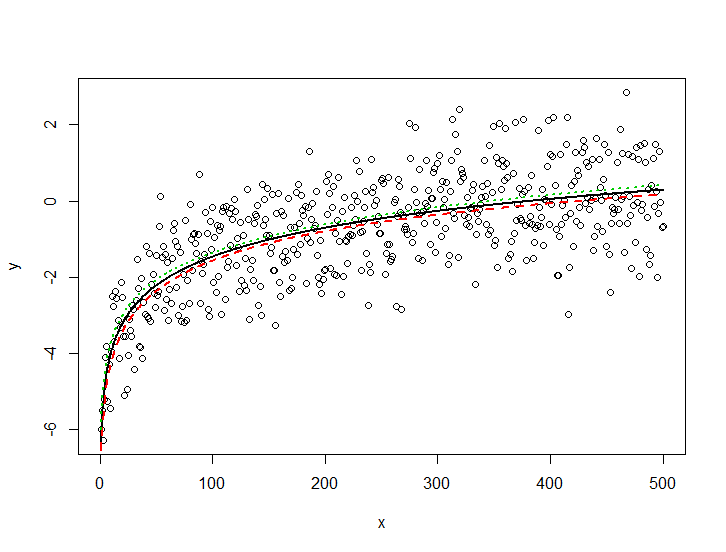
\includegraphics[scale=0.6]{logGrowth.png}
	\caption{Logarithmic growth, characterized by rapid growth initially, then a more ``linear" growth later.}
\end{figure}

\begin{figure}
	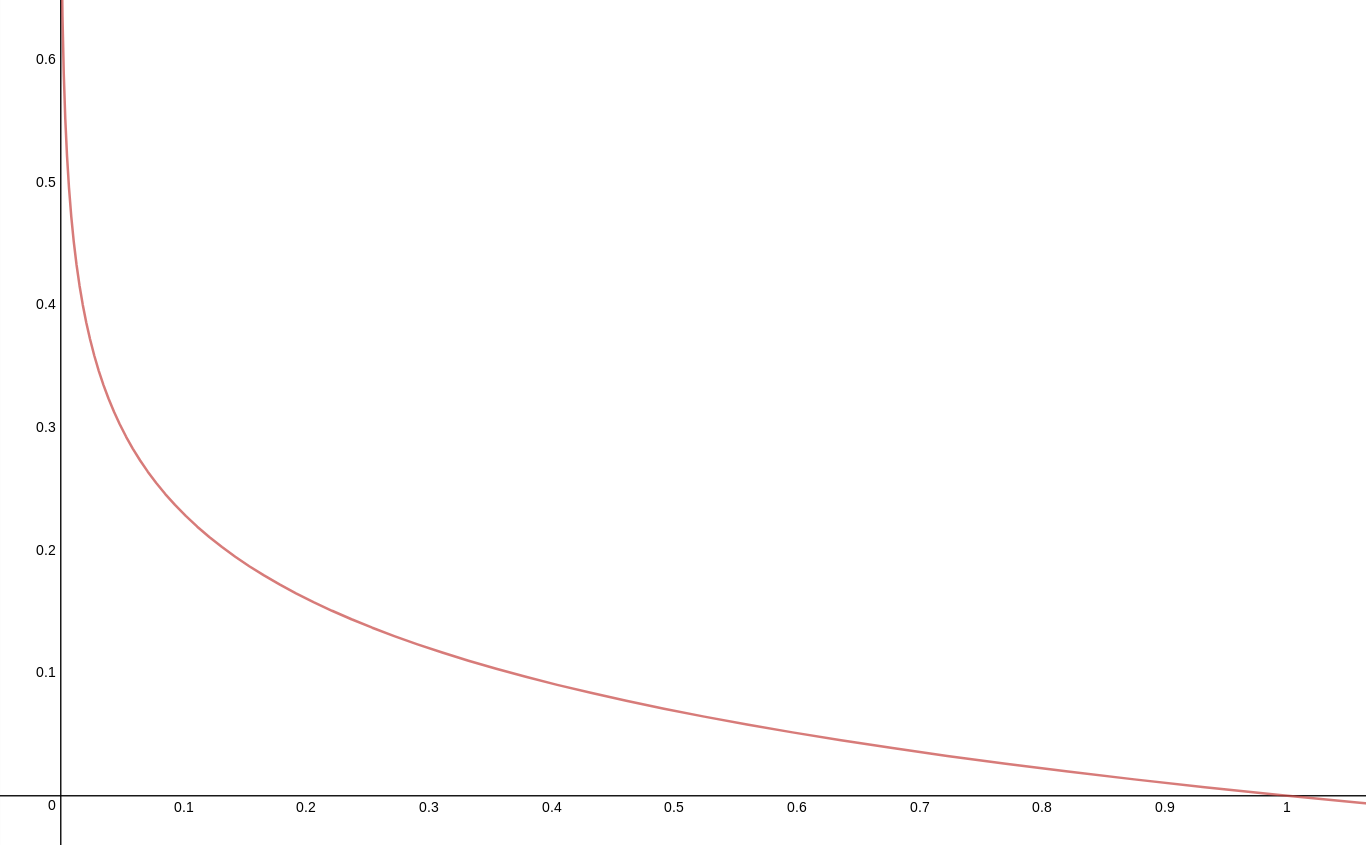
\includegraphics[scale=0.3]{logDecay.png}
	\caption{Logarithmic decay, characterized by rapid decay initially, then a more ``linear" decay later.}
\end{figure}

\end{theorem}

\begin{center} \textbf{\Large Common Logarithmic Models} \end{center}

\begin{itemize}
	\item Decibals: $d = 10 \log(P/P_0)$, where $P$ is the intensity of the sound and $P_0$ is the weakest sound a human can hear.
	\item Richter scale: $R = \log(A/A_0)$, where $A$ is the measure of the amplitude of the earthquake wave and $A_0$ is the amplitude of the smallest detectable wave.
	\item pH level: $ph = -\log([H^+])$, where $[H^+]$ is the concentration of Hydrogen.
	\item Carbon dating: $t = -\frac{1}{0.000121} \ln(r)$, where $t$ is time in years and $r$ is the percentage of Carbon in decimal form.
\end{itemize}

\begin{center} \textbf{\Large Identifying Logarithmic Models} \end{center}

For the following problems, determine if a logarithmic model would be appropriate. 


% PART 1 - Word Problems 
\begin{question}
Carlos has taken an initial dose of a prescription medication orally. The medicine is absorbed rapidly by the large intestine and absorbed slowly as it is digested otherwise. Would a logarithmic model be appropriate to describe the amount of medication, $M(t)$ (mg) in his bloodstream after $t$ hours?

$\answer[format=string]{No}$

\begin{feedback}
We see that the rate of absorption is changing as the dose makes its way through the body, so a \textit{linear} model would not be appropriate. We also do not see any mention of a \textit{direct/indirect} relationship between amount of medicine and time, so a \textit{direct/indirect variation} model would not be appropriate. So we need to decide between logarithmic and exponential. 

If we think about the absorption as it goes through the body, we would say it looks like:

slow $\rightarrow$ slow $\rightarrow$ slow $\rightarrow$ rapid \textit{(as it hits the large intestine)}

Logarithmic models describe a rapid change \textbf{early}, then a slow change later. Therefore, this situation is not appropriate for a logarithmic model.
\end{feedback}

\end{question}

\begin{question}
When discussing salary, we can talk about someone's ``\textit{[blank]}-figure salary". This is used as a rough estimate to compare salaries on a large scale. A four-figure salary would be someone making about $X,000$ dollars a year, while a six-figure salary would be someone making about $X00,000$ a year. Would be appropriate to use a logarithmic model to describe the number of figures, $n(S)$, of a person's salary in terms of their actual salary, $S$?

$\answer[format=string]{Yes}$

\begin{feedback}
Let's think about what is happening early. 

\$1 salary $\rightarrow$ $1$ figure
\$10 salary $\rightarrow$ $2$ figures
\$100 salary $\rightarrow$ $3$ figures
\$1,000 salary $\rightarrow$ $4$ figures
\$10,000 salary $\rightarrow$ $5$ figures

Small changes in the salary early (less than \$10 change in salary) move the figure by 1. As the salary increases, we need a much larger amount of salary to change the figure (to go from 4 to 5 figures, we need a change of \$9000 change in salary). In other words, we see a rapid change early, then a slower growth later, which describes a logarithmic model! 

In fact, this model is $n(S) = \log(S)+1$. If we shift our expectations for this model (since adults rarely make less than five-figure salaries), we can see that a change from $5$ figures to $6$ figures is a huge increase in standard of living!
\end{feedback}

\end{question}

% PART 2 - Graphical Data
\begin{question}
\begin{figure}
	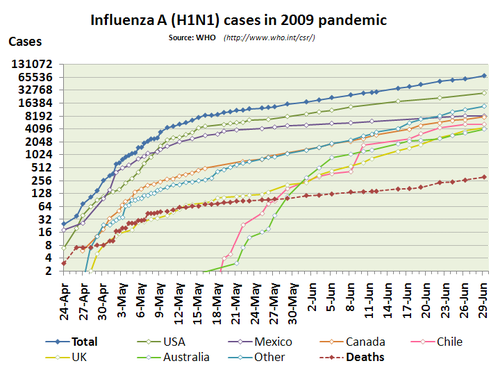
\includegraphics[scale=1]{Influenza-2009.png}
\end{figure}

Is it appropriate to model the number of Influenza A (\textit{swine flu}) cases in 2009 using a logarithmic model? 

$\answer[format=string]{Yes}$

\begin{feedback}
Logarithmic functions are useful when describing highly infectious diseases! It only takes a small number of infected individually to rapidly infect huge numbers of people. This is especially true when dealing with infections that \textbf{do not provide immunity or resistances after infection} like Influenza. 
\end{feedback}

\end{question}

\begin{question}

\begin{figure}
	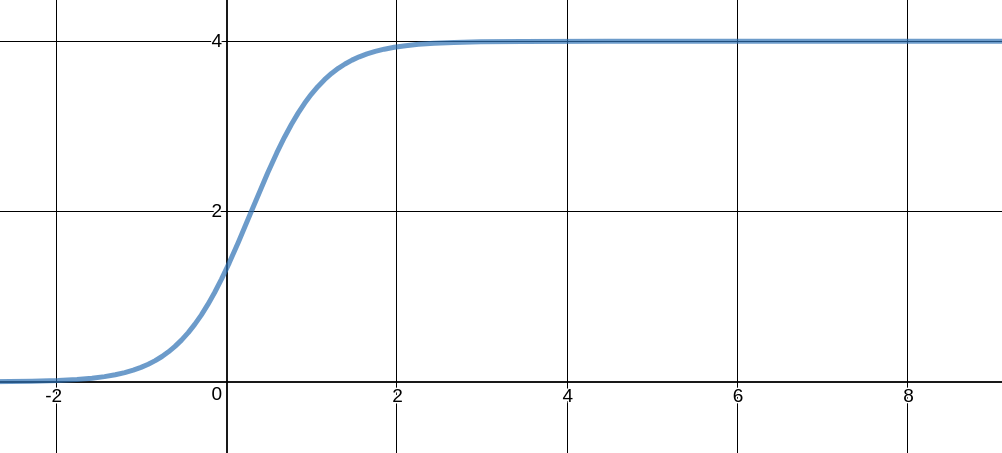
\includegraphics[scale=1]{logarithmicGrowth.png}
	\caption{A sigmodial curve.}
\end{figure}

Sigmoidal curves, like the one above, are used when dealing with population dynamics as there is normally some upper bound on the population (called the \textit{carrying capacity}). Would it be appropriate to model a sigmodial curve using a logarithmic function?

$\answer[format=string]{No}$

\begin{feedback}
You may feel tricked by this question. We see the rapid initial growth, and then a slow growth later. So why is it not appropriate to use a logarithmic function? \textbf{Because logarithmic functions grow unbounded} and this model has an upper bound. So, we'll need to refine our criteria for using a logarithmic model.
\end{feedback}
\end{question}

\begin{theorem}
	\textbf{Need for a Logarithmic Model - refined}
	
	A logarithmic model is appropriate when the quantities change rapidly \textbf{early}, then change slowly later on \textbf{without bound}. 	
\end{theorem}

\end{document}